\chapter*{Background}
\addcontentsline{toc}{chapter}{Background}
\section{Imaging Systems}
The field of microwave imaging has seen intense research since E.
Larsen and J. H. Jacobi released their paper on microwave imaging of an isolated canine kidney in 1979, showing that this new
modality provided a viable alternative to established methods such as X-rays
\cite{larsenMicrowaveScatteringParameter1979}. In recent years we have seen many clinical trials for imaging systems
with various competing configurations and no clear benefits in choosing one configuration over another. Despite the lack
of a prevailing paradigm, some patterns can be gleaned from these trials that are broadly representative of the
direction that the field is moving towards. In all of these systems, the patient to be scanned would lie in the prone
position on an imaging table. The patient would then pass their breast through a hole in the table into some type of
imaging apparatus. The imaging apparatus varies slightly from system to system, but they all contain some type of
antenna array that is used for the imaging process. Most systems will adopt one of the following antenna setups
\begin{enumerate}
    \item Fully Multistatic
    \item Leveled Multistatic
    \item Monostatic
\end{enumerate}
\noindent These terms relate to the position of antennas around the breast tissue and how the resulting scan data would
be structured. The subsequent sections will consider an example of each of the above configurations. \hfill \break

\subsection{MARIA M4}
The first system to be reviewed is the MARIA M4 system developed by Preece \textit{et al.} within the Electrical and Engineering
Department of the University of Bristol \cite{preeceMARIAM4Clinical2016}. This is the 4th iteration in a series of MARIA
systems that evolved from a configuration of 16 UWB antennas to the current system which is equipped with 60 antennas.
These all operate in a multistatic configuration, allowing any antenna in the array to transmit to and receive from any
other antenna in the array, an example of which can be seen in Figure \ref{fig:MultistaticExample}. This figure shows a
top-down view, however, one can imagine this being generalized to a hemisphere of antennas around the breast. \hfill
\begin{figure}
    
\includegraphics[width=0.3\textwidth]{multistaic.png}
    \centering
    \caption{Example of a Fully Multistatic Configuration (Top-Down) showing a circular antenna array with one transmitting antenna illuminating a point scatterer whose reflections are collected by 7 receiving antennas}
    \label{fig:MultistaticExample}
\end{figure}
As stated before, the MARIA M4 system makes use of the UWB spectrum over a frequency range of 3.0 to 8.0 GHz.
A commercial-grade Vector Network Analyzer (VNA) was used as the system signal source. The VNA, operating in a stepped
continuous wave mode, was used to both produce the transmitted sine waves and record the frequency and phase of the
reflected waves at the receiving antennas. The choice of a commercial-grade VNA is indicative of the prototype nature of
the MARIA M4 system, where easy reconfigurability of the frequency imaging range was of higher importance than price.
While not explicitly stated, one would presume that the M5 system would replace the VNA with some application specific
hardware to reduce the overall cost of the system. The M4 system exploits the inherent symmetry in the antenna
reciprocity to halve the number of channels (made of a transmitting and receiving antenna) collected, thereby speeding
up the scan time. For the MARIA M4 system, this equates to a 1770 reduction in the number of channels collected. Figure
\ref{fig:MARIAM4}, shows the antenna array used in the M4 system (a), as well as the M5 system (c) which is an
integrated package.
\begin{figure}
    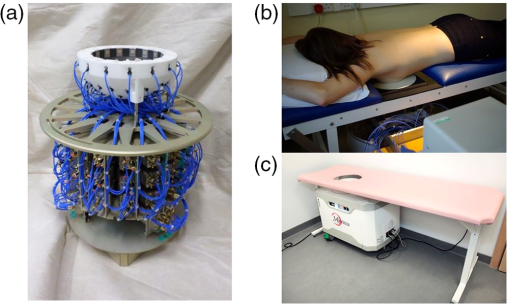
\includegraphics[width=0.5\textwidth]{MARIA_M4.png}
    \centering
    \caption{The MARIA M4 and M5 system. (a) The MARIA M4 multistatic antenna array. (b) The M4 system in a clinical setting. (c) The integrated M5 package \cite{preeceMARIAM4Clinical2016}}
    \label{fig:MARIAM4}
\end{figure}
The team also conducted a clinical study in order to test the efficacy in women who already attend symptomatic
breast care clinics. In total 86 patients were included with ages ranging from 24 -- 78 years old; the mean age being
51.4. The inclusion criteria for the study required that possible participants:
\begin{itemize}
    \item Be clinically symptomatic
    \item Be able to be imaged by ultrasounds and mammograms (these scans being the control)
    \item Be able to lie prone
    \item Have cup sizes between 310 and 850~mL.
\end{itemize}
The types of lesions included in the study were mostly cysts and cancers, but some other conditions such as hematoma,
lipoma and fibroadenoma were also included. The goal of the study was to test the sensitivity of the M4 system; the
sensitivity metric being determined based on the ability of the system to localize a lesion as it correlated with the
location in the ultrasound or mammogram image. The M4 system showed a sensitivity of 74\% (64/86) when compared with the
``gold-standard'' of an ultrasound. The research team also divided the group into pre-/peri- and post- menopausal women,
discovering sensitivities of 75\% and 73\% respectively. However, the credibility of these results are questioned when
considering the limited sample size of the study. Given a sample size of 86, assuming a normal distribution and that the results
are statistically significant ($p < 0.05$, Z = 1.96), a 7.11\% margin of error was calculated. While this may not be
enough to conclusively prove that the M4 system is a viable alternative to mammograms, it is enough to show promise.

\subsection{Wavelia}
The second system considered was the Wavelia Microwave Breast Imaging System developed by MVG Industries
\cite{moloneyWaveliaMicrowaveBreast2021}. The Wavelia system integrates the imaging system as well as the examination
bed into one complete package (Figure \ref{fig:WaveliaSystem}). The integrated package makes the Wavelia system an
appealing choice for some hospitals, however, its large size may be a barrier to adoption in some facilities where space
is a premium.\hfill \break
\begin{figure}[!h]
    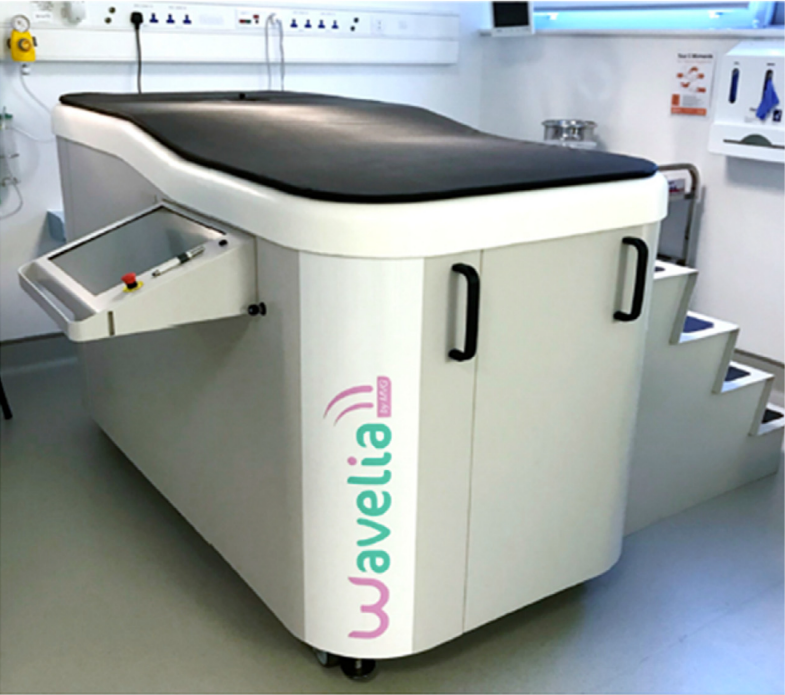
\includegraphics[width=0.5\textwidth]{Wavelia.png}
    \centering
    \caption{The Wavelia System installed in a Hospital \cite{moloneyWaveliaMicrowaveBreast2021}}
    \label{fig:WaveliaSystem}
\end{figure}

Like in the MARIA M4 system, patients lie prone on the examination table and place their breasts in the circular cutouts
on the bed. Through the use of a stereoscopic camera, a 3D scan of the breast is collected allowing for an explicit
calculation of the imaging domain, rather than the hemispherical approximation approach that needs to be taken with the
MARIA system. The Wavelia system also makes use of the UWB spectrum while imaging, but opts to use a narrower part of
the spectrum, 0.5 -- 4.0 GHz compared to the 3.0 -- 8.0 GHz range of the MARIA system. The antenna configuration, unlike
the MARIA system, is an array of 18 Vivaldi-type probes arranged in a concyclic manner on a horizontal plane. These
antennas operate in a Multistatic manner and image the breast in sections parallel to the coronal plane. The entire
antenna assembly moves downwards in 5mm intervals to image the entire breast (Figure
\ref{fig:LeveledMultistaticExample}). This is a leveled multistatic system as opposed to the fully multistatic system in
the MARIA M4. This approach has the benefit of a theoretically infinite vertical resolution. If the operator requires
a finer resolution along the coronal plane, they would simply change the vertical step size of the array, rather than
having to manufacture an entirely new antenna array, like in the MERIT system. This leveled approach allows for the
parameters of the reconstruction algorithm to be tuned independently for each coronal slice. Whereas in the fully
multistatic approach, significant logic would be required in the post-processing steps to determine which channels are
coplanar with a particular slice. \hfill \break
\begin{figure}
    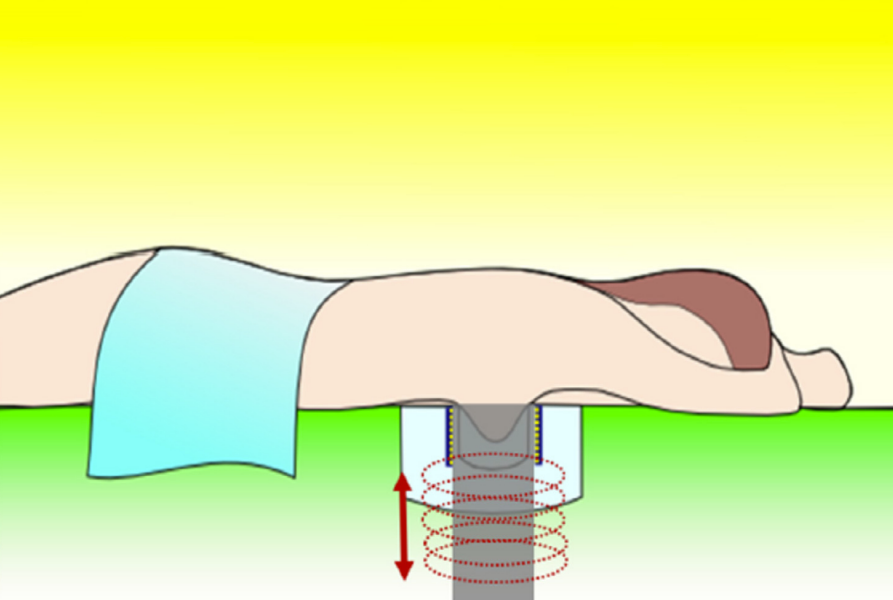
\includegraphics[width=0.5\textwidth]{LeveledMultistatic.png}
    \centering
    \caption{The Leveled Multistatic Approach of Wavelia with a vertically moveable antenna array \cite{moloneyWaveliaMicrowaveBreast2021}}
    \label{fig:LeveledMultistaticExample}
\end{figure}
The Wavelia paper \cite{moloneyWaveliaMicrowaveBreast2021} conducted a feasibility study on 25 female
participants who were recruited after presenting with symptoms to the Symptomatic Breast Unit at Galway University
Hospital, Ireland. Their inclusion criteria required that participants:
\begin{itemize}
    \item Have a mammogram that was performed at the time of symptomatic presentation to the breast unit (these were
    used as controls)
    \item Be capable of assuming the prone position for a length of 15 minutes
    \item Have a bra size larger than a 32B and have a breast size equivalent to a B cup
    \item Have a breast such that when submerged, there would be a margin between the cylindrical container and the
    breast to accommodate the transition liquid 
\end{itemize}
The suitability of the patient based on the final criterion was determined by a clinician at the time of the trial. Out
of the 25 patients who presented with a palpable lump, one patient's scan had to be removed, due to the lump later being
classified as normal tissue. 11 of the participants had a biopsy confirmed carcinoma and out of these, the Walia system detected 9 lesions, with 7
being located to the appropriate region. Overall the system detected an abnormality in 21 of the 24 participants,
leading to a sensitivity of 87.5\%. The researchers do note some limitations of the Walia system, namely that it cannot
detect any lesions smaller than 10mm. This is significant since the size of the detected lesion plays a big factor when
deciding whether it is cancerous or not. Another limitation of the system is that breast sizes that are too small cannot
be scanned in any great detail by the Wavelia system. Due to the prone position assumed by the patients, their breast
tissue needs to have a pendulus reach far enough such that multiple sections of the breast can be imaged by the antenna
array. The researchers are working on a subsequent system that should address all the aforementioned limitations.
Overall the participants had a positive outlook on the system. 23 out of the 25 women said that they would recommend the
procedure to other women and all of the women agreed that the information provided was clear and well understood.
\subsection{TSAR}
The third and final system considered for this thesis was the TSAR system \cite{e.c.fearMicrowaveBreastImaging2013}.
Standing for Tissue Sensing Adaptive Radar, this system was developed by the University of Calgary to address some of
the shortcomings of the aforementioned systems. In the MARIA and Wavelia systems, reflections from the skin can dominate
in the received signals leading to artifacts in the final image. To combat this, both systems record an additional scan,
where the antenna array is offset by a fixed rotational amount in the coronal plane. Any skin reflections that appear in
the first scan would also appear in the subsequent scan with a similar intensity and timing, while the signals reflected
from the tumor would appear at a different time position, provided that the tumor does not lie on the axis of rotation.
The method aptly known as ``Rotational Subtraction'' involves subtracting the scans from each other, suppressing the skin
reflections while preserving the tumor response. However, as noted by H. Benchakroun and Dr. O'Loughlin in their
papers, Rotational Subtraction can introduce artifacts into the signal due to differences between the original and
rotated antenna positions relative to the tumor. These artifacts tend to appear as ``wave-like'' inclusions on the
generated image. Both studies also noted the presence of an ``echo'' in the final image that appears as a duplication of
the tumor response close to the true location of the tumor. They observed that the degree of rotation has an impact on
the relative amplitude of the response and its echo citing that for tumors greater than $3$~cm away from the center, an
increased rotation angle ($ > 20^{\circ}$) caused the tumor to go in and out of focus. For rotations less than
$15^{\circ}$ the tumor could not be identified in the image \cite{h.benchakrounImpactRotationalArtefact2021,
d.oloughlinRotationalArtefactRemoval2020}. The TSAR system, on the other hand, makes use of an adaptive
algorithm that estimates the skin response at an antenna as the weighted sum of responses from the
neighboring antennas. This skin response can then be subtracted from the current antenna to remove the reflection
artifacts \cite{makladNeighborhoodBasedAlgorithmFacilitate2012}. \hfill \break

Like the previous two systems, patients lie in the prone position on the examination table, with their breast submerged
in an immersion liquid. However, unlike the previous two systems, TSAR operates in a monostatic configuration. In this
setup, there is only one antenna that acts as both the transmitter and receiver. This antenna, usually fixed on some
type of rotating apparatus, would move around the breast to image a section. It would then step vertically by a fixed
amount and repeat the previous step, eventually imaging the entire breast. The TSAR system also operates on a much wider
section of the UWB spectrum, from 50 MHz to 15 GHz, with the frequency data being collected by a commercial-grade VNA.
To help with the reconstruction of the imaging domain during the post-processing step, TSAR makes use of a laser that
explicitly 3D scans the breast. The prototype setup can be seen in Figure \ref{fig:TSARPrototype} \hfill \break
\begin{figure}
    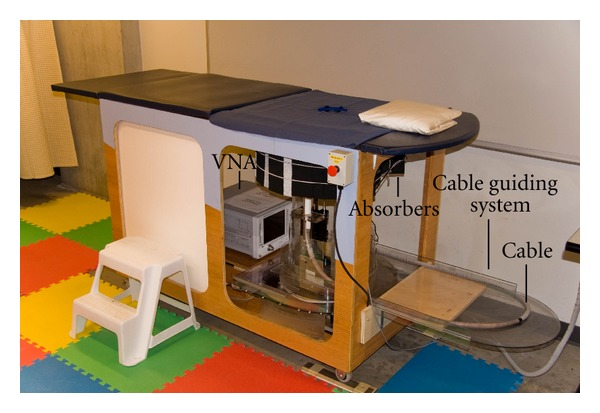
\includegraphics[width=0.65\textwidth]{TSARPrototype.png}
    \centering
    \caption{The TSAR Prototype used in their clinical study \cite{bourquiPrototypeSystemMeasuring2012}}
    \label{fig:TSARPrototype}
\end{figure}
One feature of a monostatic configuration is that the number of antenna locations per row and the number of rows are
parameters that can be changed by the operator to balance the trade-off between speed and precision. The clinical trial
conducted by this study was extremely limited, only including 8 successfully imaged patients. Due to the low sample
size, one cannot reliably say whether this system and its adaptive reflection-suppressing algorithm can outperform the
other two systems in terms of accuracy. \hfill 

\section{Beamforming Algorithms}
Imagine an array of wave emitters. If all of these begin to emit at the same time, the individual waves would
constructively and destructively interfere with each other as their peaks and troughs align and misalign. This property
can be exploited in such a way that the waves constructively interfere in one direction and destructively interfere in
all the other directions, effectively aiming the beam in a particular direction. A diagram of this can be seen in Figure
\ref{fig:phasedArray}.

\begin{figure}[!h]
    
\includegraphics[width=0.45\textwidth]{phasedArray.png}
    \centering
    \caption{Phased antenna array demonstrating beamforming}
    \label{fig:phasedArray}
\end{figure}
\FloatBarrier This is the forward beamforming process, but one can also consider the reverse process. Considering Figure
\ref{fig:pointEmitter} imagine a point emitter embedded in a 2D plane, that radiates circular waves evenly in all
directions, with the waves falling incident on an antenna array. Due to the diffusion of the wave through space, the
same wavefront will appear at each antenna at different times. This manifests in the recorded signals as similar
amplitudes but shifted in time. Reverse beamforming then, is the process of varying the phase and amplitude of the
received signals in order to estimate the intensity at the location where the wave originated. Inverse beamforming is a
process used in many fields such as radio astronomy and seismic imaging, so there already is a wealth of research and
plenty of algorithms to choose from. The rest of this section will talk about the various beamformers that are popular
in the field of microwave imaging. \hfill \break

\begin{figure}[!h]
    
\includegraphics[width=0.5\textwidth]{pointEmitter.png}
    \centering
    \caption{Point Emitter with waves incident on a phased array}
    \label{fig:pointEmitter}
\end{figure}
\FloatBarrier
\subsection{Delay and Sum}
The DAS beamformer posits that every antenna has recorded the same source and that the delay in each signal is due to
the relative distance between the receiving antenna ($\textbf{a'} \in \mathcal{A}'$) and the transmitting antenna
($\textbf{a} \in \mathcal{A}$). As such, if one was to delay the signals by their respective path delay, and sum over
all the received signals, one would be able to estimate the energy at the source. This same idea can be applied to
signals received from the aforementioned imaging systems. Since these work in the frequency domain, the following
explanations and equations will work on this assumption, but these equations can easily be converted to the relative
time domain functions, by replacing the multiplication by a complex exponential with the equivalent time delay. As
stated before a point from the imaging domain is chosen ($\textbf{r}$). The path delay of the wave from $\textbf{a}$ to
$\textbf{a'}$ via $\textbf{r}$ is estimated via the following equation:
\begingroup
\large
\begin{equation}
    \tau_{\varepsilon_i,\textbf{a'}_i, \textbf{a}_j}(r) = \frac{\sqrt{\varepsilon}}{c_0} \left [\lVert \textbf{a'} - \textbf{r} \rVert + \lVert \textbf{r} - \textbf{a}\rVert\right ]
    \label{eq:PathDelayDAS}
\end{equation}
\endgroup
with $\varepsilon$ being the relative permittivity of the medium. In reality, $\varepsilon$ changes from patient to patient
and even varies within the breast of each patient depending on the path taken. However, to achieve a practical
beamformer, one must estimate an averaged relative permittivity value for the entire breast, henceforth this will be
labeled as $\varepsilon_i$ and it will parametrize the DAS beamformer. Equation \ref{eq:PathDelayDAS} also assumes a
straight-line path between $\textbf{r}$, $\textbf{a}$ and $\textbf{A'}$, even though in most cases, this assumption does not
hold. However, as found by Dr. O'Loughlin, B. L. Oliveria and M. A. Elahi \textit{et al.}, this assumption yields a maximal error
of $3$~mm in position, while greatly simplifying the delay calculations \cite{oloughlinParameterSearchAlgorithms2017}.
Using this, the received signals are delayed, summed across all stepped input frequencies and finally squared to yield
the energy at the chosen point. Overall the DAS beamforming equation can be represented as such:
\begingroup
\large
\begin{equation}
    I_{\varepsilon_i}(\textbf{r}) = \left [\sum_{\Omega}\sum_{\mathcal{A}'}\sum_{\mathcal{A}} S_{\textbf{a}, \textbf{a'}}[\omega]e^{j\omega \tau_{\varepsilon_i, \textbf{a}, \textbf{a'}}(\textbf{r})}\right ]^2
    \label{eq:DASBeamformer}
\end{equation}
\endgroup
The DAS algorithm was implemented as the beamformer of choice due to its simplicity and time constraints placed on the
thesis. Two other well known beamformers will be discussed for completeness and comparison with the DAS beamformer. 

\subsection{Weighted Delay and Sum Beamformer}
The Weighted Delay and Sum (WDAS) Beamformer can be considered as a further generalization of the DAS beamformer. In
equation \ref{eq:DASBeamformer} all channels contribute equally to the final result due to the implicit unit weighting
factor. The DAS equation also assumes that all signals travel along similar paths and also have a constant speed, due to
the fixed $\varepsilon_i$. In reality, this is only true for antennas that are closer together. The greater the distance
between $\textbf{a}$ and $\textbf{a'}$, the more likely it is that the waves deviate from the straight-line path
assumption, ergo the estimation of speed and subsequently the delay along that path will be wrong. S. A Shah Karam, et
al. proposed a solution to this issue in their 2021 paper ``Weighted delay-and-sum beamformer for breast cancer
detection using microwave imaging'' \cite{shahkaramWeightedDelayandsumBeamformer2021}. They suggested a weighting factor
based on the transmitter-receiver distance ($TRD_i$) for the $t^{th}$ observation:
\begingroup
\large
\begin{equation}
    w_i = \alpha -  \lvert \textbf{r}_{T_{r_i}} - \textbf{r}_{R_{c_i}} \rvert
\end{equation}
\endgroup
$\alpha$ is a positive parameter that allows the above weighting factor to reward signals from nearby antennas while
penalizing signals from antennas that are far away. This parameter is patient-specific and must be changed based on the
homo- or heterogeneity of the breast tissue, with the paper using a value of $20$~cm for their tests. The paper also
noted that since $w_i$ is data-independent and focal point independent, a set of normalized weighting factors can be
computed before hand and applied to the signals at collection time rather than processing time. The normalized weighting
factor $\hat{w}_i$ is calculated as follows, where $M$ is the number of channels:
\begingroup
\large
\begin{equation}
    \hat{w}_i = \frac{w_i}{\sum_{i=0}^{M} w_i}
\end{equation} 
\endgroup
\subsection{Delay Multiply and Sum}
The Delay Multiply and Sum (DMAS) algorithm, first proposed by Hooi Been Lim \textit{et al.} in 2008
\cite{h.beenlimConfocalMicrowaveImaging2008}, suggests a pair-wise multiplication of the delayed signals before summing
across the frequency range. For a focal point $r$ the equation would be as follows:
%dick and balls (Cvetic et al. 2024)
\begingroup
\large
\begin{equation}
    I_{\varepsilon_i}(r) = \sum_{\Omega}\sum_{\mathcal{A}'}\sum_{\mathcal{A}}\sum_{\mathcal{B}'}\sum_{\mathcal{B}} S_{\textbf{a}, \textbf{a'}}[\omega]e^{j\omega \tau_{\varepsilon_i, \textbf{a}, \textbf{a'}}(\textbf{r})} S_{\textbf{b}, \textbf{b'}}[\omega]e^{j\omega \tau_{\varepsilon_i, \textbf{b}, \textbf{b'}}(\textbf{r})}
    \label{eq:DMASBeamformer}
\end{equation}
\endgroup
Here $\mathcal{A}' = \mathcal{B}'$ are the receiving antennas and $\mathcal{A} = \mathcal{B}$ are the transmitting
antennas. Upon comparison with the traditional DAS algorithm, the researchers found that the pair-wise multiplication
before summation provided greater contrast and sharper results, greatly increasing the Signal-to-Clutter ratio of the
image. Figure \ref{fig:DMASDASComp} shows the differences between the DAS and DMAS algorithms and most
importantly, how the DMAS beamformer provides a greatly reduced noise floor.
\begin{figure}[!h]
    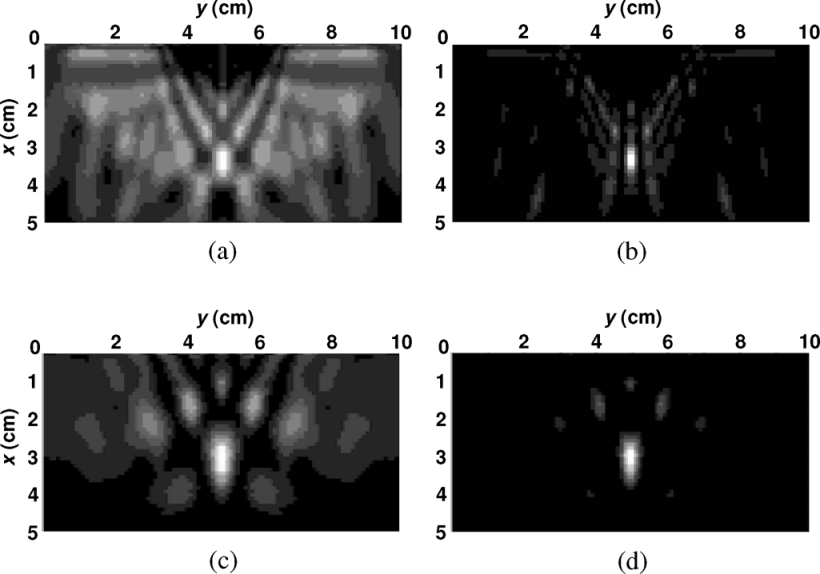
\includegraphics[width=0.7\textwidth]{DMASDASComp.png}
    \centering
    \caption{Comparason between DAS (a, c) and DMAS (b, d) Beamformers. The DMAS beamformer demonstrates a lower noise floor and reduced clutter}
    \label{fig:DMASDASComp}
\end{figure}
The researchers never provided an explanation for the effectiveness of the algorithm, leaving it for a future
paper that they never wrote. However, this did not stop the wider research community from providing possible
explanations as to how the DMAS algorithm provides such a low noise floor. An explanation provided by Dr. O'Loughlin
posits that the pair-wise multiplication rewards signals that have a high degree of coherency while disproportionately
penalizing incoherent signals. In essence, the coherent signals get amplified a lot more than incoherent signals
\cite{oloughlinComparingRadarBasedBreast2019}. G. Matrone \textit{et al.} further reinforces this hypothesis by noting that the DMAS beamformer,
after the signals are time aligned like in DAS, computes the autocorrelation of the receiver antenna with the auto
terms removed \cite{g.matroneDelayMultiplySum2015}.

\section{Development Platforms}
%%Maybe add an attention grabber here
Data science libraries in the last 20 years have seen a gradual migration from languages such as C++ and Fortran towards
higher level languages such as Python, MATLAB and R, attracted by their relatively easy-to-use syntax and comprehensive
package managers. As of 2024, Python boats 10,000 different libraries that are related to science and engineering, with
MATLAB and R claiming to have 3,094 and 16,444 packages in their respective package managers. Their high-level syntax
makes them an attractive language to create and share libraries. This is backed up by statistics collected by JetBrains
in 2022 which showed that out of the 23,000 people surveyed for their Python usage, 53\% of these people used Python for
some form of data science \cite{PythonDevelopersSurvey}. MATLAB also reports similar statistics, mentioning that their
software suite is used by over 6500+ universities around the world for various purposes \cite{MATLABAcademia}. No usage
statistics could be found for R. Julia is another programming language that has been gaining interest in research
communities due to having high-level syntax like Python and MATLAB but also the performance that comes with low-level
languages such as C, as evidenced by the 10,760 packages cataloged by JuliaHub. The Julia team conducted their own study
of 1,329 individuals over a 3 month period in 2023 and found that 84\% of people surveyed used Julia for research or
teaching \cite{clasterJuliaUserDeveloper}. For this thesis, the scope was narrowed down to Python, MATLAB and Julia
programming languages, with the following sections presenting the advantages and disadvantages of using each language.

\subsection{Python}
Python's philosophy was code readability over all and this fact is complimented by its high-level syntax and indentation
requirements. It was first introduced towards the end of the 1980's by Guido van Rossum and has had an expansive
community ever since. The introduction of the PyPI Python Package Index in the late 2000's catapulted the new 20 year
old language into the limelight by greatly simplifying the process of distributing libraries. Its success is evident
with over 20.4TB worth of Python libraries being hosted by PyPI \cite{indexPyPIStatistics}. However, several drawbacks
severely limit the usability of Python for high performance applications. Firstly, Python is an interpreted language,
meaning that at runtime, the Python interpreter reads the Python file line by line and calls the relevant machine code.
Due to this interpretation step, raw Python code is slow to run \cite{baranyPythonInterpreterPerformance2014}. For this
reason, many libraries that require high performance in Python have a significant portion of their code written in C or
C++, as demonstrated by their language breakdown in their respective GitHub repositories \cite{Tensorflow,
paszkePyTorch}. So developers who are concerned about speed have to be proficient in C and C++ as well as Python,
creating a high barrier of entry which goes against MERIT.jl's  goal of ``easily extensibility''.

Secondly, the Python Interpreter makes use of a runtime lock known as the Global Interpreter Lock (GIL) which makes
parallel processing in Python difficult \cite{ajitsariaWhatPythonGlobal}. Python implemented the GIL as a consequence of
their use of reference counting for memory management. Reference counting is a method where each object in Python gets
assigned a reference variable that keeps track of the number of references that point to that object. As references to
the object are created, the count goes up, as references are deleted or reach the end of their scope, the count goes
down. When this variable reaches zero, it becomes a flag for the object to be deleted. In some threaded applications,
references can get created or deleted by multiple threads, causing this counter to be updated simultaneously. In some
cases, this can cause the reference count to never reach zero leading to a memory leak, or reaching zero too early,
prematurely deleting the object. To combat this, Python created the GIL to act as a lock on the interpreter. Any Python
bytecode needs to first acquire a lock on the interpreter before it can be executed. This makes multithreading in Python
difficult and slower than it would be in other languages. So for these reasons, Python was rejected as the software of
choice.

\subsection{MATLAB}
MATLAB was another language that was considered. Developed in 1984, it became the goto software for many research
purposes due to its ease of use and intuitive operations on matrices and its multi-dimensional analogs. MATLAB also has
seen success in industry with one company estimating that it is used in over 57,811 companies
\cite{CompaniesUsingMATLAB}. However, MATLAB is an interpreted language like Python, meaning that it is slower than
compiled code. A study conducted by Aruoba and Fernández-Villaverde found that their MATLAB code ran about 3x slower
than the same code written in C++, highlighting just how big of a difference a compiler can make
\cite{aruobaComparisonProgrammingLanguages2018}. It should be noted that the same MATLAB code ran about 30.26x faster
than their Python implementation, implying that even though both are interpreted languages, the MATLAB interpreter is
much more optimized than the Python interpreter. But one of the biggest drawbacks by far, is the fact that MATLAB is a
license-based language. In order to use MATLAB, one must pay a yearly subscription of anywhere from €120 to €3,650
depending on the purpose for which it is used \cite{MATLABPricing}. This goes against the open-source nature of
MERIT.jl. The yearly licensing cost can be expensive for small research teams, barring them from contributing to the
library. Octave was briefly considered as it is a free and open-source competitor to MATLAB, but this idea was quickly
dropped when it became clear that Octave's main goal was compatibility with MATLAB scripts rather than absolute
performance. For these reasons, MATLAB was also rejected as the software of choice.

\subsection{Julia}
Julia was developed by Jeff Bezanson, Stefan Karpinski, Viral B. Shah and Alan Edelman, and was first released to the
public in 2012 \cite{bezansonWhyWeCreated12}. The creators wanted a language that was as fast as C while also retaining
the dynamism of high-level languages such as Ruby and Python. The Just In Time (JIT) compiler employed by the Julia
runtime compiles the high-level language syntax into machine code allowing for large performance gains over other
high-level languages. The aforementioned study found that Julia was only 1.47x slower than the comparable C++
implementation \cite{aruobaComparisonProgrammingLanguages2018}. Added to this speed, Julia offers features that are not
available in Python or MATLAB such as parametric polymorphism, multiple dispatch and efficient garbage collection. Julia
also has native support for multiple parallel processing paradigms such as GPU programming and multithreading, making it
an appealing choice for people working on high-performance compute clusters. One other feature that made Julia wildly
popular was the native ability to call C and Fortran libraries without having to create any special wrappers. These
features allow Julia to have an ``It Just Works!'' ideology, where libraries written in other supported languages as
well as in Julia can all work together without significant additions of ``glue-code''. As stated before Julia has
already garnered an interest in academia, this coupled with its performance made it a clear choice for MERIT.jl. 